\documentclass[a4paper]{article}

%% Language and font encodings
\usepackage[english]{babel}
\usepackage[utf8x]{inputenc}
\usepackage[T1]{fontenc}
\usepackage{subfig}

%% Sets page size and margins
\usepackage[a4paper,top=3cm,bottom=2cm,left=3cm,right=3cm,marginparwidth=1.75cm]{geometry}

%% Useful packages
\usepackage{amsmath}
\usepackage{graphicx}
\usepackage{wrapfig}
\usepackage{float}
\usepackage{amsfonts}
\graphicspath{ {./img/} }
\usepackage[colorinlistoftodos]{todonotes}
\usepackage[colorlinks=true, allcolors=blue]{hyperref}

\title{\vspace{-2.5cm}Estimation of Hurst Parameter of Mono-fractal signals\\ EE-678, Wavelets, Prof. V.M. Gadre}
\author{Agrim Gupta, Saurabh Pinjani, Asim Ukaye \\ PhD Supervisor: Shivam Bhardwaj, MTech Mentor: Harsh Solanki}

\begin{document}
\maketitle

\begin{abstract}
In the main course assignment, we explored self similar signals and how to estimate them using techniques in wavelet domain. A good starting point was PCA Eigenspectrum paper [1] by Li et al. The proposed method works good for the H parameter in range (0.5,1) and doesn't scale up with sample size as well. Our proposed algorithm using detail coefficients of DWT improves upon these shortcomings. In addition, we studied and implemented paper on "Bayesian Estimation of $\gamma$ for 1/f signals" and experimented with different wavelet basis for the same, which hadn't been attempted by the authors before
\end{abstract}

\section{Introduction}

\subsection{Fractals}
In mathematics, a self-similar object is exactly or approximately similar to a part of itself  i.e. the whole has the same shape as one or more of the parts. Self-similarity is a typical property of fractals.

\begin{figure}[h]
    \centering
    \subfloat[Triangular Fractals]{{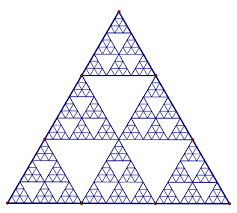
\includegraphics[width=5cm]{fractals_1.png} }}%
    \qquad
    \subfloat[Close-up of a Romanesco broccoli]{{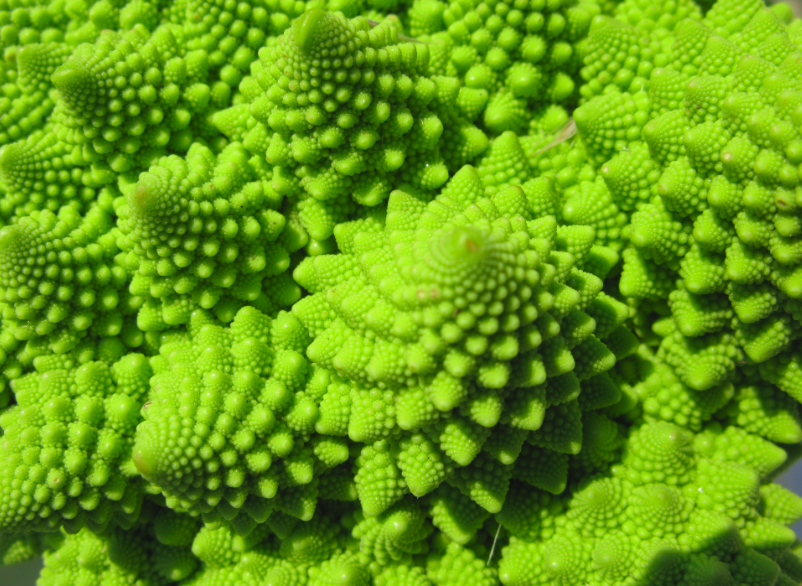
\includegraphics[width=5cm]{fractals_2.png} }}%
    \caption{Examples of fractals are abound.}%
    \label{fig:example}%
\end{figure}

\subsection{Self-Similar Signals}
A random process is said to be self-similar if its statistics are invariant to compressions and dilations of the waveform in time i.e. its statistical properties don’t change with scaling. In mathematical terms
$$x(t) \equiv a^{-H}x(at)$$
Here the ‘H’ in the exponent is called the Hurst Parameter. This parameter is used to characterize such self similar random processes. We will be looking at methods of extraction of this parameter going forward in this report.

\begin{figure}[h]
  \begin{minipage}[c]{0.67\textwidth}
    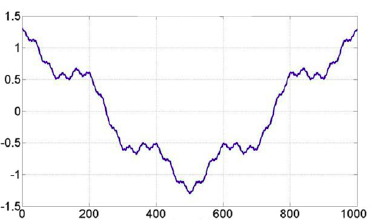
\includegraphics[width=\textwidth]{self_sim.png}
  \end{minipage}\hfill
  \begin{minipage}[c]{0.3\textwidth}
    \caption{
       Weierstrass signal is an example of a self-similar signal. If we cut out the part of the signal from t=400 to t=600, the part is similar to the whole.
    } 
  \end{minipage}
\end{figure}

In this report we will be primarily dealing with two particular classes of self similar signals :
(i) Fractional Brownian Motion  (ii) $\frac{1}{f}$ processes

\section{Self-similar Signals studied}
\subsection{Fractional Brownian Motion (fBm) signal}
fBm, a generalization of Brownian motion, is a continuous-time Gaussian process BH(t) on [0, T], which starts at zero, has expectation zero for all t in [0, T]​.
​Unlike classical Brownian motion, the increments of fBm need not be independent and can be positively or negatively correlated. The degree of correlation is what characterises the process and is captured in the Hurst parameter(H). When H assumes a value lower than 0.5 the increments are negatively correlated and for values above 0.5 they are positively correlated. If H is 0.5 the steps are uncorrelated and hence the fBm becomes a vanilla brownian motion.
It has the following covariance function \cite{DBLP:journals/tit/TewfikK92}:
$$R_{B_H}(s,t)=E[B_H(s)B_H(t)]=\frac{V_H}{2}(|s|^{2H}+|t|^{2H}+|s-t|^{2H})$$
where $V_H=var[B_H(1)]=\frac{-\Gamma(2-2H)cos(\pi H)}{\pi H(2H-1)}$

We saw various forms of the covariance functions in \cite{DBLP:journals/tit/TewfikK92},\cite{DBLP:journals/tsp/LiHCZ09} and \cite{FBM_var}. The most general version is presented above. 

\begin{figure}[h]
  \begin{minipage}[c]{0.6\textwidth}
    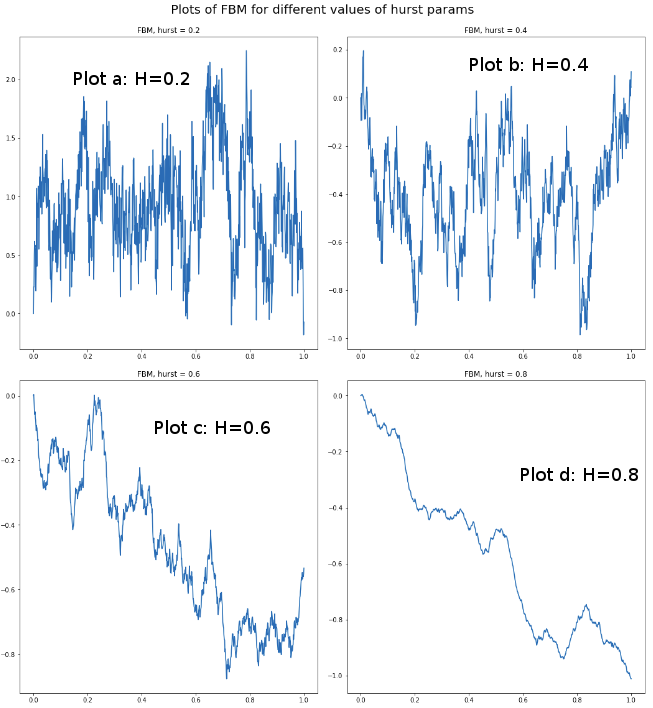
\includegraphics[width=\textwidth]{fbm_H2.png}
  \end{minipage}\hfill
  \begin{minipage}[c]{0.4\textwidth}
    \caption{
       The Hurst parameter fully characterizes a monofractal signal such as fBm. The graphs above
illustrate this point. In graph (a) H=0.2. Hence the incremental steps are negatively correlated
and hence the graph is tremulous. However in graph (d) where H=0.8 the graph is quite smooth
due to the positive correlation between subsequent steps. So therefore as we move from graph
(a) to (d) the graph gets smoother with an increasing Hurst parameter.
    } 
  \end{minipage}
\end{figure}

\subsection{1/f Processes}
This is a class of self similar signals that possess a power spectrum obeying the following law:
$$S(\omega)=\frac{\sigma_x^2}{|\omega|^\gamma}$$
where $\gamma=2H+1$. $\gamma$ typically lies between 0 and 2.
It is generally convenient to extend the notion of l/f processes to include nearly 1/f processes that are defined as having power spectra bounded according to:
$$\frac{k_1}{|\omega|^\gamma} \leq S(\omega) \leq \frac{k_2}{|\omega|^\gamma}$$
where $k_1$ and $k_2$ satisfy $0 < k_1 \leq k_2 < \infty $

\section{Extraction of Hurst Parameter in fBm}
Since the Hurst parameter characterises the fBm, its extraction from a given signal is a problem of great relevance. This has been studied in existing literature. The method discussed in literature is discussed below. We will also be analyzing its shortfalls and domain of applicability.

\subsection{H parameter estimation using PCA Spectrum (Li et al. 2009) \cite{DBLP:journals/tsp/LiHCZ09}}
\begin{wrapfigure}{r}{8cm}
\vspace{-15pt}
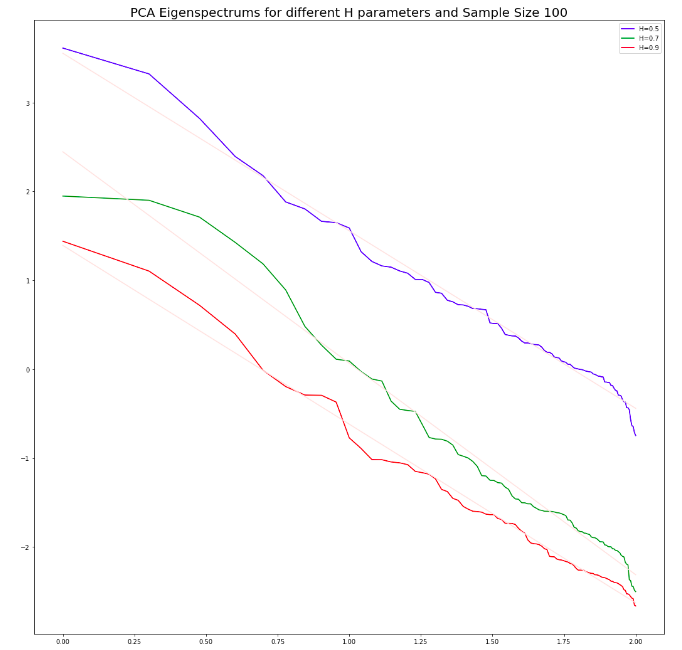
\includegraphics[width=8cm]{Li_1.png}
\end{wrapfigure} 
A method to estimate the hurst parameter from the PCA eigenspectrum of a FBM signal was proposed. The PCA eigenspectrum of the autocovariance matrix of FBM signal is linear in log log scale, and the slope is indicative of the Hurst parameter. The method was theoretically proved by showing equivalence of eigenvalues arising from discrete K-L expansion and autocovariance matrix. However this method is plagued with certain issues:
\begin{itemize}
\item This method works for signals with H in the range (0.5,1). This is a serious shortcoming as many signals in real life have negative correlation.
\item As sample size increased the difference between the estimated and actual value of Hurst increases. Ref. Figure below.
\end{itemize}
\begin{figure}[h]
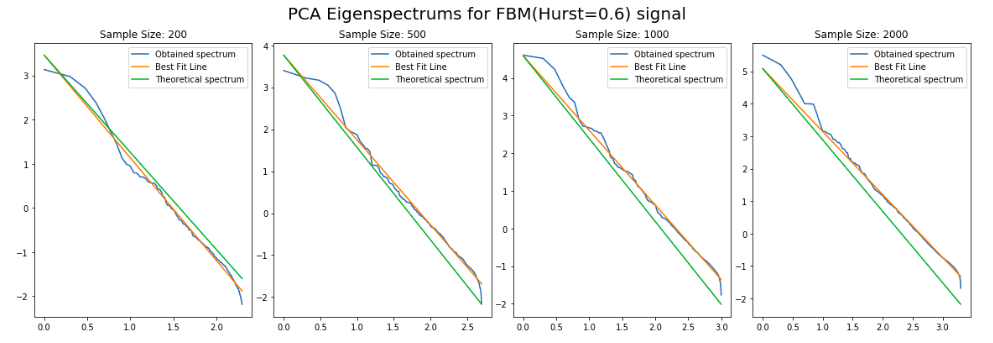
\includegraphics[width=\textwidth]{Li_2.png}
\caption{As Sample Size increases, deviation between actual slope and expected slope increases}
\end{figure}

\subsection{H parameter estimation using Eigenspectrum of Detail coefficients}
Instead of forming autocovariance matrix of the FBM signal, we first take DWT of the FBM signal. Then we use the detail coefficients (high pass branch) to form the autocovariance. Then we plot the eigenspectrum of the modified autocovariance matrix in log log scale. However, instead of looking at the slope we look at the y-intercept. We can map the y-intercept (which is nothing but the highest eigenvalue) to the Hurst parameter.
Now to judge the effectiveness of the method we look at the graph for the PCA spectrum method reported in literature. One can clearly see that separability of the curves have increased in our method. Hence our method is clearly advantageous.

\begin{figure}[H]
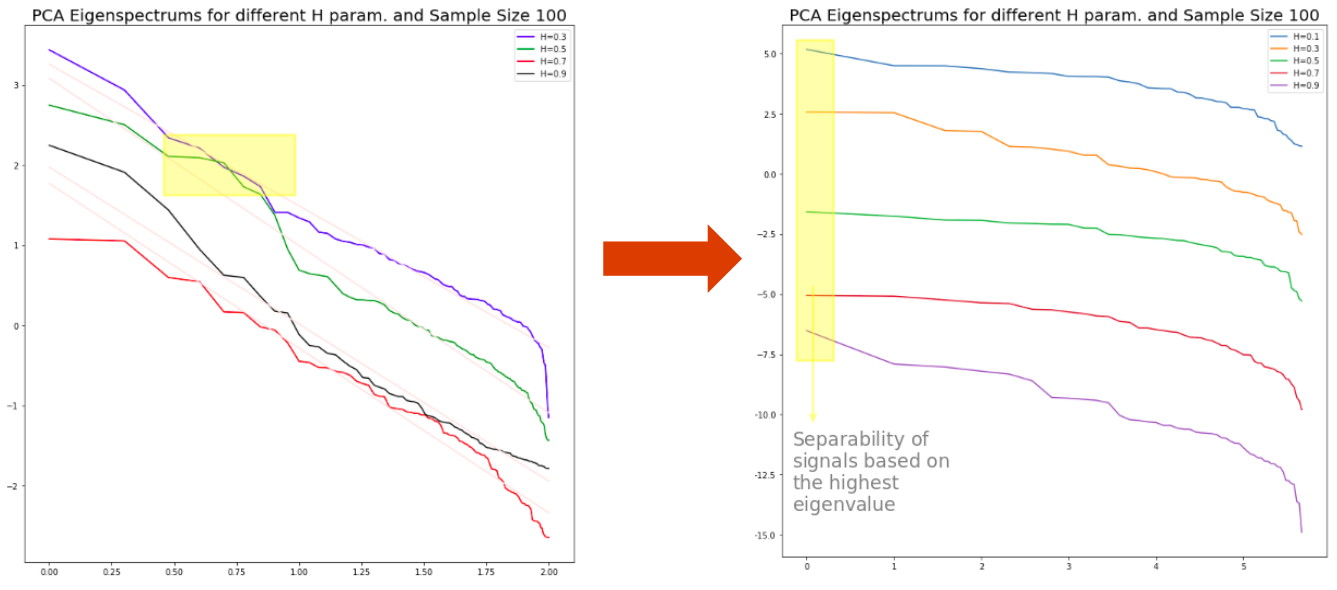
\includegraphics[width=\textwidth]{dwt_1.png}
\caption{Separability of curves generated by different H increases when eigenspectrum of detail coefficients is plotted}
\end{figure}

\begin{wrapfigure}{r}{7cm}
\vspace{-30pt}
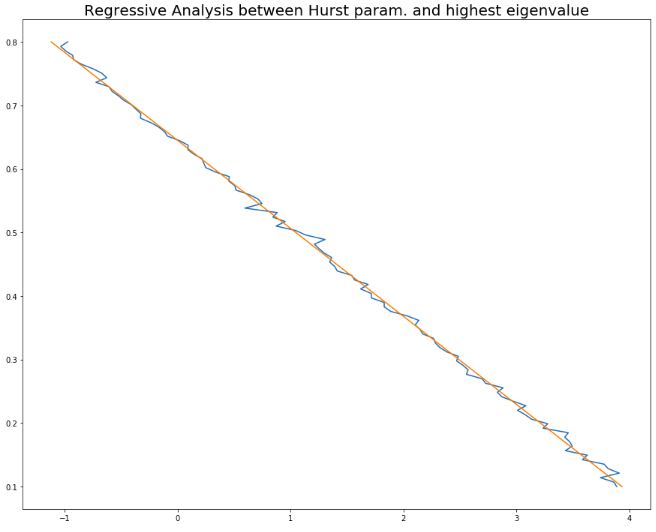
\includegraphics[width=7cm]{dwt_lin.png}
\vspace{-30pt}
\end{wrapfigure} 
Next step is to fit in the y highest eigenvalues against the Hurst parameter of the signal. A linear fit suffices and gives sufficiently good results, indicating the linear relationship between Hurst parameter and highest eigenvalue.  It is clear from the graph that this method gives a fairly accurate estimate of the Hurst parameter, even for hurst parameters in the range (0,0.5) which could not be obtained accurately via the PCA eigenspectrum method proposed by Li et al.
\\
\\
\\

\begin{wrapfigure}{l}{7cm}
\vspace{-30pt}
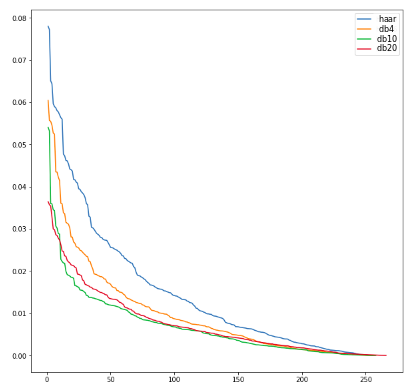
\includegraphics[width=7cm]{hyp.png}
\caption{Hyperbolic decay of eigenvalues\\}
\vspace{-30pt}
\end{wrapfigure}
Another Interesting observation was that when eigenspectrum is plotted straightaway and not in log log scale, we see a hyperbolic decrease. The paper by H. Tewfik and M. Kim\cite{DBLP:journals/tit/TewfikK92} reported a similar hyperbolic decrease, but for the autocorrelation after taking DWT (but not for the eigenvalues). As vanishing moments increase, the hyperbolic decrease is steeper, which was also observed in \cite{DBLP:journals/tit/TewfikK92}. This indicates a deeper connect between eigenspectrum and direct DWT.\\ \\ \\

\pagebreak
\subsubsection{Mathematical analysis of the proposed method}
\begin{itemize}
\item Using the fact that the highest eigenvalue($\lambda_1$1) of the Auto covariance matrix with all positive entries is $1+(M-1)\sum_{i=1}^M(p*R(p))$ \cite{Eigen}, mathematical analysis of the results obtained was attempted. To make all the entries in the Auto covariance matrix positive,  $|min_p(R(p))|$ can be added. Hence, the following formula was obtained, from which linearity when plotted in log log scale can be explained.​
$$\lambda_1 = 1+(M-1)(\frac{1}{\frac{M(M-1)}{2}}\sum_{p=1}^{M-1}pR[p]+|min_{p}(R[p])|)$$
\item However, to obtain the exact values of slope, we need to solve the minimization problem formally and account in for a more accurate expression for R[0], which has been left as a potential future work.​
\item Explaining this via Discrete KL Expansion was also attempted, but it did not give fruitful result. Another issue faced was with various forms of R[k]. Using approximations to R[k] results in counterfeit results, and as a future work expression used for R[k] should be improved upon to explain the obtained results completely​
\end{itemize}
\subsubsection{Future Work Possible}
\begin{itemize}
	\item Completing the analysis by solving the optimization problem directly and calculating the highest eigen value. However, there are 2 issues with this approach, since firstly, in presence of noise, the problem will become probabilistic and may be untrackable, and secondly, the optimization problem may not have a closed form. Moreover, the analysis done will be just for the highest eigenvalue and not for the full spectrum.
	\item Given the drawbacks of the approaches considered, proving the results using discrete K-L expansion might be the correct way to proceed. The paper by Li et al \cite{DBLP:journals/tsp/LiHCZ09} presented an unusual proof which connects the discrete KL expansion to the PCA method. The proof however isn't very general and can't be readily applied to other basis functions \cite{5447734}. Li et al, in January 2018, although have replied to the comment and have come up with a stronger proof concerning with Reisez basis and other such tools, and it will be a good exercise to try and generalize it to Haar wavelet \cite{response}.
	\item Since we are using Detail coefficients here, it makes sense to try and generalize it across the scales via wavelet packet transform. \cite{4127049} by Wang et al also have proposed estimating Hurst parameter using wavelet packet transform instead of DWT. 
\end{itemize}
\section{Estimation of Fractality parameters (H \& $\gamma$) for \\1/f processes}
In our assignment we also aimed to study and implement \cite{DBLP:journals/tsp/WornellO92} presented by Wornell and Oppenheim. This paper shows a robust, computationally efficient and consistent iterative algorithm to estimate Fractality Parameters (H), ​and variance estimates of 1/f processes using wavelet expansion
By implementing the ideas and algorithms proposed in this paper we were able to understand the wavelet domain analysis of fractals through implementation. We also aimed at replicating some of the results proposed in the paper and observe and comment on certain parts which the paper did not discuss, such as the effect of choice of wavelet basis on estimates of H.

The ultimate goal of this activity was to research the possibility of extending the framework (given for 1/f processes) of this paper to f-ARIMA processes.

\subsection{Outline of the paper}

The paper can be summarized in 4 parts: A background on concepts involved, Problem Formulation \& Iterative Algorithm, Verification \& Signal Reconstruction,and Simulations \& Results.
\subsubsection{Background}
The paper discusses the lack of research on 1/f processes and their parameterization. $1/f$ processes are described in the first part of this report. The problem is to find the best estimate for $\gamma$ for a given $1/f$ signal if embedded in a Gaussian White Noise. \\
The suggested algorithm uses wavelet decomposition to convert the problem in Wavelet Domain. A section of the paper is devoted to the definition of Orthonormal Wavelet Decomposition of Signals. The paper generally uses Daubechies-5 wavelet for most of the simulations. The proposed algorithm uses the the wavelet-based Karhunen-Loéve (KL)-like expansions for 1/f processes. It is shown that one can construct a class of nearly $1 /f$ processes using wavelet expansions in terms of uncorrelated transform coefficients having the variance progression:
$$var\ x_n^m = \sigma^22^{-\gamma m}$$

where $\gamma$ is the exponent of the nearly $1/f$ spectrum, and $\sigma^2$ is a positive constant proportional to $\sigma_x^2$.

\subsubsection{Problem Formulation \& Algorithm}

Let us suppose we have observations $r(t)$ of a zero mean Gaussian $1/f$ process $x(t)$ embedded in zero-mean additive stationary white Gaussian noise $w(t)$ that is statistically independent of $x(t)$.

$$r(t) = x(t) + w(t)\qquad -\infty<t<\infty $$

From this data, the Wavelet coefficients are obtained as such:
$$ r_n^m = \int_{-\infty} ^\infty \psi_n^m(t)r(t)dt.$$
We use a DWT where the finite set representing all the scales is given by:
$$\mathfrak{M} = \{ m_1,m_2,\ldots, m_M \} $$
And at each scale m, the of available coefficients is given by:
$$\mathfrak{N}(m) = \{ n_1(m),n_2(m),\ldots, n_{N(m)}(m) \} $$
Hence, the available data is:
$$r = \{ r_n^m \in \mathfrak{R}\} = \{ r_n^m, m\in \mathfrak{M},n\in \mathfrak{N}(m) \} $$
Exploiting the wavelet decomposition’s role as a whitening filter for 1/f processes, and using the fact that the wnm are independent of the xnm and are decorrelated for any wavelet basis, the resulting observation coefficients
$$r_n^m = x_n^m + w_n^m $$
can be modeled as mutually independent zero-mean, Gaussian random variables with variance
$$var\ r_n^m = \sigma^2_m =\sigma^2 \beta^{-m} + \sigma^2_w$$
Where,
$$\beta = 2^\gamma $$
Thus, the parameter set defined below is the one that is to be estimated.
$$\Theta = (\beta , \sigma^2, \sigma^2_w)$$

The likelihood function for the above parameter set is expressed as:
$$\mathfrak{L}(\Theta) = p_r(r;\ \Theta) = \prod _{m,n\in \mathfrak{R}} \frac{1}{\sqrt[]{2\pi \sigma _m^2}}\ \text{exp} \bigg [-\frac{(r_n^m)^2}{2\sigma^2_m}\bigg]$$
for which the log-likelihood function is
$$L(\Theta) = -\frac{1}{2}\sum_{m,n\in \mathfrak{R}}\bigg \{ \frac{1}{\sigma_m^2}(r_n^m)^2+ \text{ln} (2 \pi \sigma_m^2 ) \bigg \}  $$
Equivalently,
$$L(\Theta) = -\frac{1}{2}\sum_{m \in \mathfrak{M}}N(m)\bigg \{ \frac{\hat{\sigma_m^2}}{\sigma_m^2}+ \text{ln} (2 \pi \sigma_m^2 ) \bigg \}  $$

Where the M sample variances given by
$$\hat{\sigma_m^2} = \frac{1}{N(m)} \sum_{n \in \mathfrak{N}(m)}(r_n^m)^2 $$
summarize the aspects of the data required in the estimation.

\subsubsection{E-M Algorithm}
In order to estimate $\Theta$, the log likelihood function $L(\Theta)$ needs to be maximized. The paper solves this problem for 3 different cases:  $\sigma_w^2$ :unknown, $\sigma_w^2$ :known and, $\sigma_w^2$ = 0. Here I am just highlighting the first case and showing the steps of the algorithm proposed which effectively achieves the goal of maximizing the function. The detailed proof of the algorithm is given in the Appendix of the paper. Estimates of parameters  $\beta ,\sigma^2, \sigma_w^2$ generated at $l^{th}$ step are denoted as $\hat{\beta}^{(l)} ,\hat{\sigma}^{2(l)}, \hat{\sigma}_w^{2(l)}$. \\
\underline{\textbf{E step:}} This step reduces to estimating the noise and signal portions of the wavelet coefficient variances at each scale m using current estimates of the parameters.
$$ S_m^w(\hat{\Theta}^{(l)}) = A_m(\hat{\Theta}^{(l)}) + B_m^w(\hat{\Theta}^{(l)})\hat{\sigma}_m^2 $$
$$ S_m^x(\hat{\Theta}^{(l)}) = A_m(\hat{\Theta}^{(l)}) + B_m^x(\hat{\Theta}^{(l)})\hat{\sigma}_m^2 $$
where,


$$A_m(\hat{\Theta}^{(l)}) = \frac{\hat{\sigma}_w^{2(l)}\cdot \hat{\sigma}^{2(l)} [\hat{\beta}^{(l)}]^{-m} }{\hat{\sigma}_w^{2(l)} + \hat{\sigma}^{2(l)} [\hat{\beta}^{(l)}]^{-m}} $$
$$B^w_m(\hat{\Theta}^{(l)}) = \bigg ( \frac{\hat{\sigma}_w^{2(l)}}{\hat{\sigma}_w^{2(l)} + \hat{\sigma}^{2(l)} [\hat{\beta}^{(l)}]^{-m}} \bigg )^2$$
$$B^x_m(\hat{\Theta}^{(l)}) = \bigg (\frac{\hat{\sigma}^{2(l)} [\hat{\beta}^{(l)}]^{-m} }{\hat{\sigma}_w^{2(l)} + \hat{\sigma}^{2(l)} [\hat{\beta}^{(l)}]^{-m}} \bigg )^2 $$
\underline{\textbf{M step:}}  This step reduces to using these signal and noise variance estimates to obtain the new parameter estimates.

$$ \hat{\beta}^{(l+1)} \leftarrow \sum_{m \in \mathfrak{M}} C_m N(m)S_m^x (\hat{\Theta}^{(l)}) \beta^m = 0 $$
$$ \hat{\sigma}^{2(l+1)} = \frac{\sum_{m \in \mathfrak{M}} N(m)S_m^x (\hat{\Theta}^{(l)})[\hat{\beta}^{(l+1)}]^m }{\sum_{m \in \mathfrak{M}} N(m)}$$
$$ \hat{\sigma}_w^{2(l+1)} = \frac{\sum_{m \in \mathfrak{M}} N(m)S_m^w (\hat{\Theta}^{(l)}) }{\sum_{m \in \mathfrak{M}} N(m)}$$
where, 

$$C_m \overset{\triangle}{= } \frac{m}{\sum_{m \in \mathfrak{M}} m N(m)} - \frac{1}{\sum_{m \in \mathfrak{M}} N(m)} $$
This concludes the problem formulation and the algorithm.

\subsubsection{Verification \& Signal Reconstruction}
The verification part shows the convergence of the algorithm by determining the Cramer-Rao bounds on the obtained estimates. We are omitting this section as it does not contribute towards the implementation of the paper. 
The second part shows the use of classical estimation theory and the fact that the input signal and the noise are jointly Gaussian and uncorrelated in order to draw an elegant formula to express the most optimal estimate of the 1/f signal as:
$$ \hat{x}(t) = \sum _{m,n} \hat{x}_n^m \psi_n^m (t) = \sum _{m,n} \bigg [ \frac{\sigma^2 \beta^{-m}}{\sigma^2 \beta^{-m} + \sigma^2_w } \bigg ] r_n^m \psi_n^m (t)$$

\subsection{Simulation and Comparison with Published Results}
\subsubsection{Implementation in MATLAB :}
\begin{itemize}
\item Generate a $1/f$ process $x(t)$, with known parameters $(\gamma, N)$ 
\item Find signal parameters $(\beta , \sigma^2)$ ; $\beta = 2^\gamma $
\item Add Gaussian White Noise of known SNR.  ($r(t) = x(t) + w(t)$)
\item Obtain wavelet coefficients for noisy signal ($r_n^m$)
\item Feed the variance of coefficients ($\sigma ^2$) of noisy signal in the E-M algorithm 
\item Obtain estimated signal parameters $$ \hat{\Theta}_{ML} = [\hat{\beta}_{ML}, \hat{\sigma}^2_{ML} , \hat{\sigma}^2_{w, ML}]$$
\item Establish the effect on estimation error with input parameters:
\begin{enumerate}
\item Resolution
\item Choice of Wavelet basis
\item SNR
\end{enumerate}
\item Reconstruct the original signal using estimated parameters.
\end{itemize}

\subsubsection{Spectral Density of the Signal.}

\begin{wrapfigure}{r}{8cm}
\vspace{-15pt}
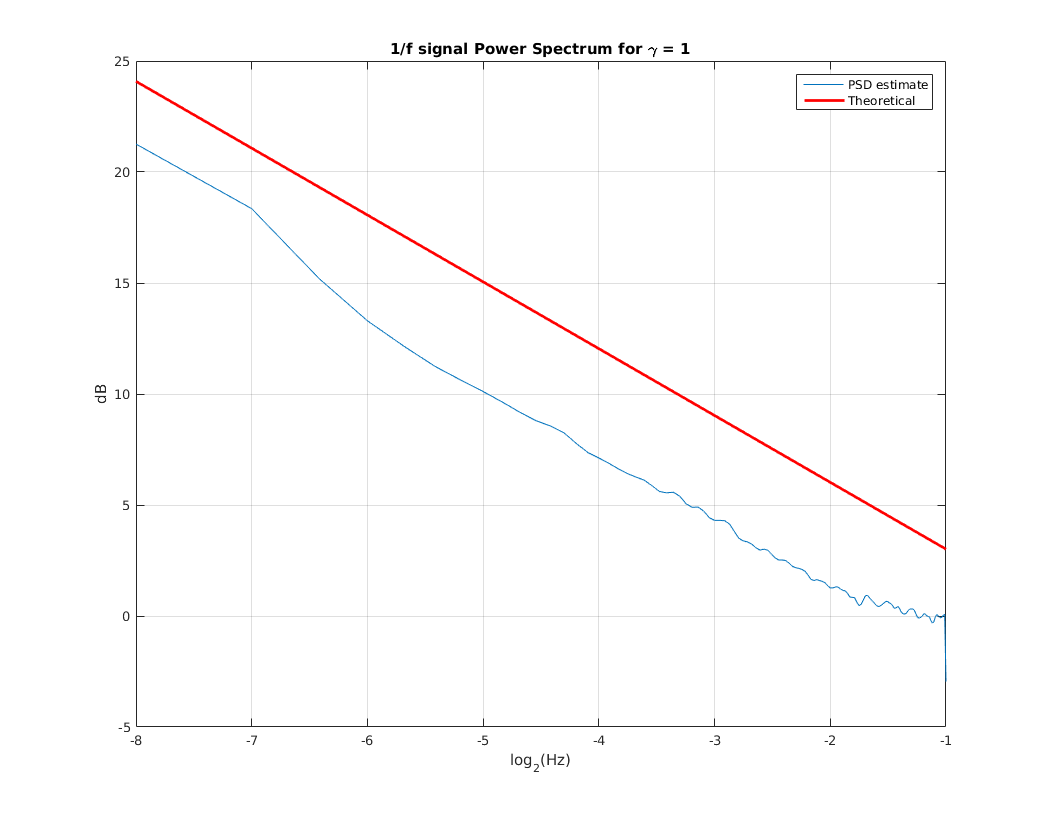
\includegraphics[width=8cm]{spectrum.png}
\caption{Power Spectral Density}
\vspace{-100pt}
\end{wrapfigure} 

\underline{\textbf{Comments:}}
\begin{itemize}
\item The power spectral density curve was obtained for the generated signal with $\gamma$ = 1 and N = 65536 ($2^{16}$) samples. 
\item The red curve shows the theoretical decay of a 1/f process on a log-log plot
\item From the estimated power spectrum, it can be seen that the slope of the input signal closely matches with that of the theoretical curve

\end{itemize}
\vspace{2 cm}

\subsubsection{Estimation of $\gamma , \sigma^2 $ using linear regression}

\begin{wrapfigure}{r}{8cm}
\vspace{-15pt}
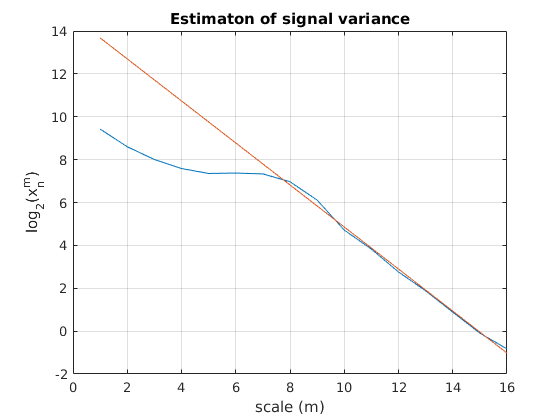
\includegraphics[width=8cm]{regression.png}
\label{fig:regr}
\caption{Linear fit of K-L expansion}
\vspace{-70pt}
%\vspace{-pt}
\end{wrapfigure} 

\underline{\textbf{Comments:}}
\begin{itemize}
\item Fig. 8 is a log-log plot of the wavelet coefficients of the input signal x(t), versus the scale (m) .
\item This plot gives us the value of $\gamma, \sigma^2 $ using the relation:
$$var\ x_n^m = \sigma^22^{-\gamma m}$$
\item The slope of the linear fit gives $-\gamma$, and the y-intercept gives an estimate of $\sigma^2 $.
\item An interesting observation while performing simulations shows that the curve is highly non-linear for lower values of $m$ (coarser scales), but is linear for finer scales. As a result of this observation for multiple sample sizes, the linear fit was obtained considering the higher values of $m$ only, i.e. for $m > M/2$. Where M is the highest scale available.

\end{itemize}
\subsubsection{Absolute Error in estimation of $\gamma$ for varying SNR. (Fig.\ref{fig:gamma_snr})}
Sample size (N) = 2048; Wavelet Basis = Daubechies 5th order

\begin{figure}[h]
    \centering
    \subfloat[Published Results]{{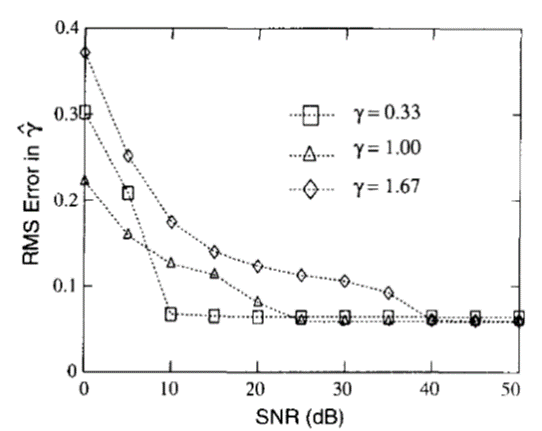
\includegraphics[width=0.46\textwidth]{gam_snr.png} }}%
   \qquad
    \subfloat[Our Results]{{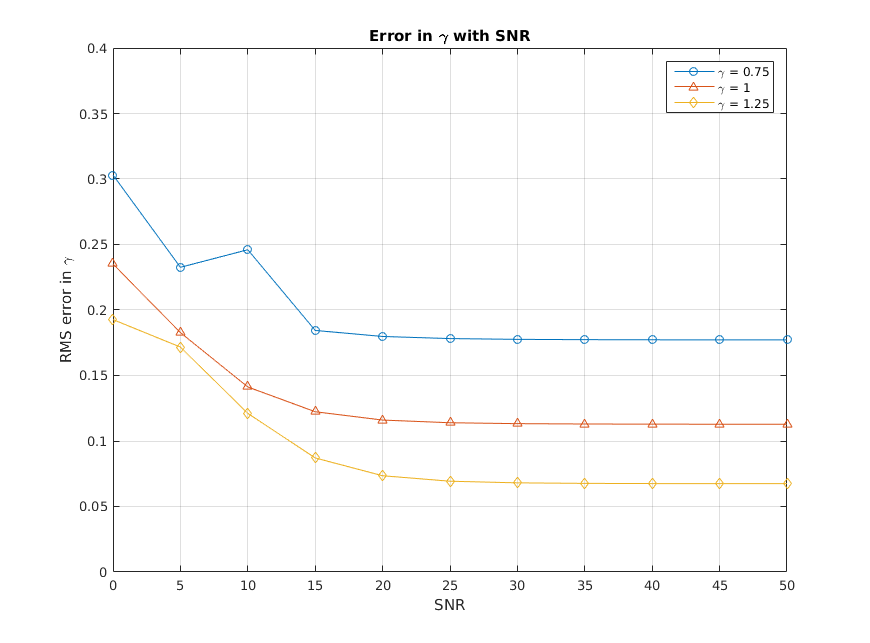
\includegraphics[width=0.46\textwidth]{gamma_snr.png} }}%
    \caption{Error in $\gamma$ with SNR}%
    \label{fig:gamma_snr}%
\end{figure}

\underline{\textbf{Comments and Inference:}}
\begin{itemize}
\item The error convergence with SNR is seen in both the results. 
\item An interesting observation is made in our results that the error values we obtained were higher for lower values of $\gamma$ as opposed to the published results. (Possible reasons mentioned in the conclusion) 
\end{itemize}

\subsubsection{Absolute Error in estimation of $\gamma$ for varying Sample Size (Fig.\ref{fig:gamma_n})}
SNR = 20 dB; Wavelet Basis = Daubechies 5th order

\begin{figure}[h!]
    \centering
    \subfloat[Published Results]{{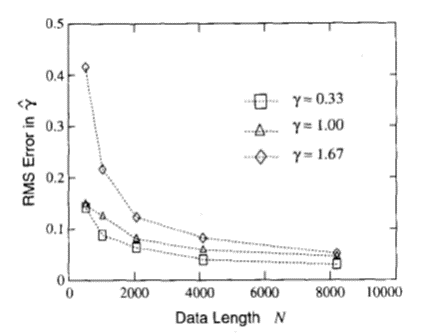
\includegraphics[width=0.46\textwidth]{gam_n.png} }}%
   \qquad
    \subfloat[Our Results]{{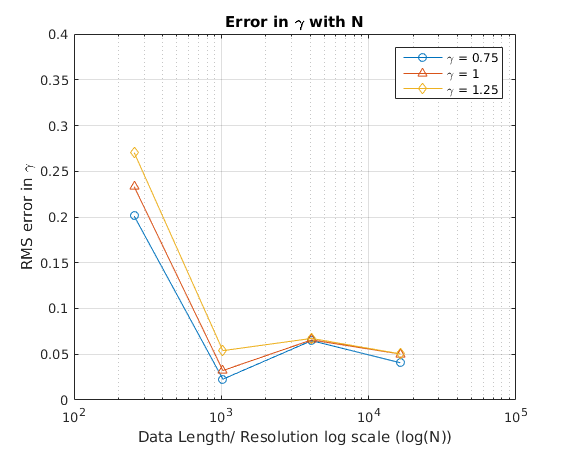
\includegraphics[width=0.46\textwidth]{gamma_n.png} }}%
    \caption{Error in $\gamma$ with Data Length (N)}%
    \label{fig:gamma_n}%
\end{figure}

\underline{\textbf{Comments and Inference:}}
\begin{itemize}
\item The error convergence with increasing sample size is seen in both the results.
\item The trend with varying $\gamma$ is also similar in both the results. 
\item An observation is made in our results that the error values anomalously drop for the data point at N = 1024. (Possible reasons mentioned in the conclusion) 
\end{itemize}

\subsubsection{Signal Reconstruction (See Fig. 11 and Fig. \ref{fig:reconstr_sim})}
Sample Size = 65536 ; SNR = 0 dB ; Wavelet basis = DB-5; $\gamma$ = 1.67 for published results; \\$\gamma$ = 1 for our results.

\begin{wrapfigure}{r}{7cm}
\vspace{-20pt}
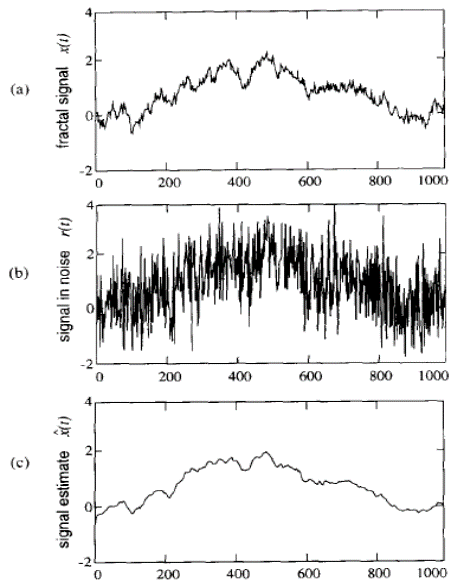
\includegraphics[width=7cm]{reconst.png}
\label{fig:reconst}
\caption{Published Results of Signal Reconstruction}
\vspace{-180pt}
%\vspace{-pt}
\end{wrapfigure}
\underline{\textbf{Comments and Inference:}}
\begin{itemize}
\item As can be seen in both the results that the reconstructed signal estimate loses a large amount of its high frequency variations in the process of de-noising.
\item We used values of $\gamma$ = 1 (or close to 1) in all our simulations because of the high deviation from 1/f behaviour at higher or lower values of $\gamma$. This was seen in the linear fitting curve mentioned in Fig. 8. This is mostly attributed to the signal generating process used by us which is a standard MATLAB function [\textit{dsp.ColoredNoise()}] which is mainly suited for standard values of $\gamma$ only.
\end{itemize}
\vspace{4 cm}
\begin{figure}[ht]
\centering
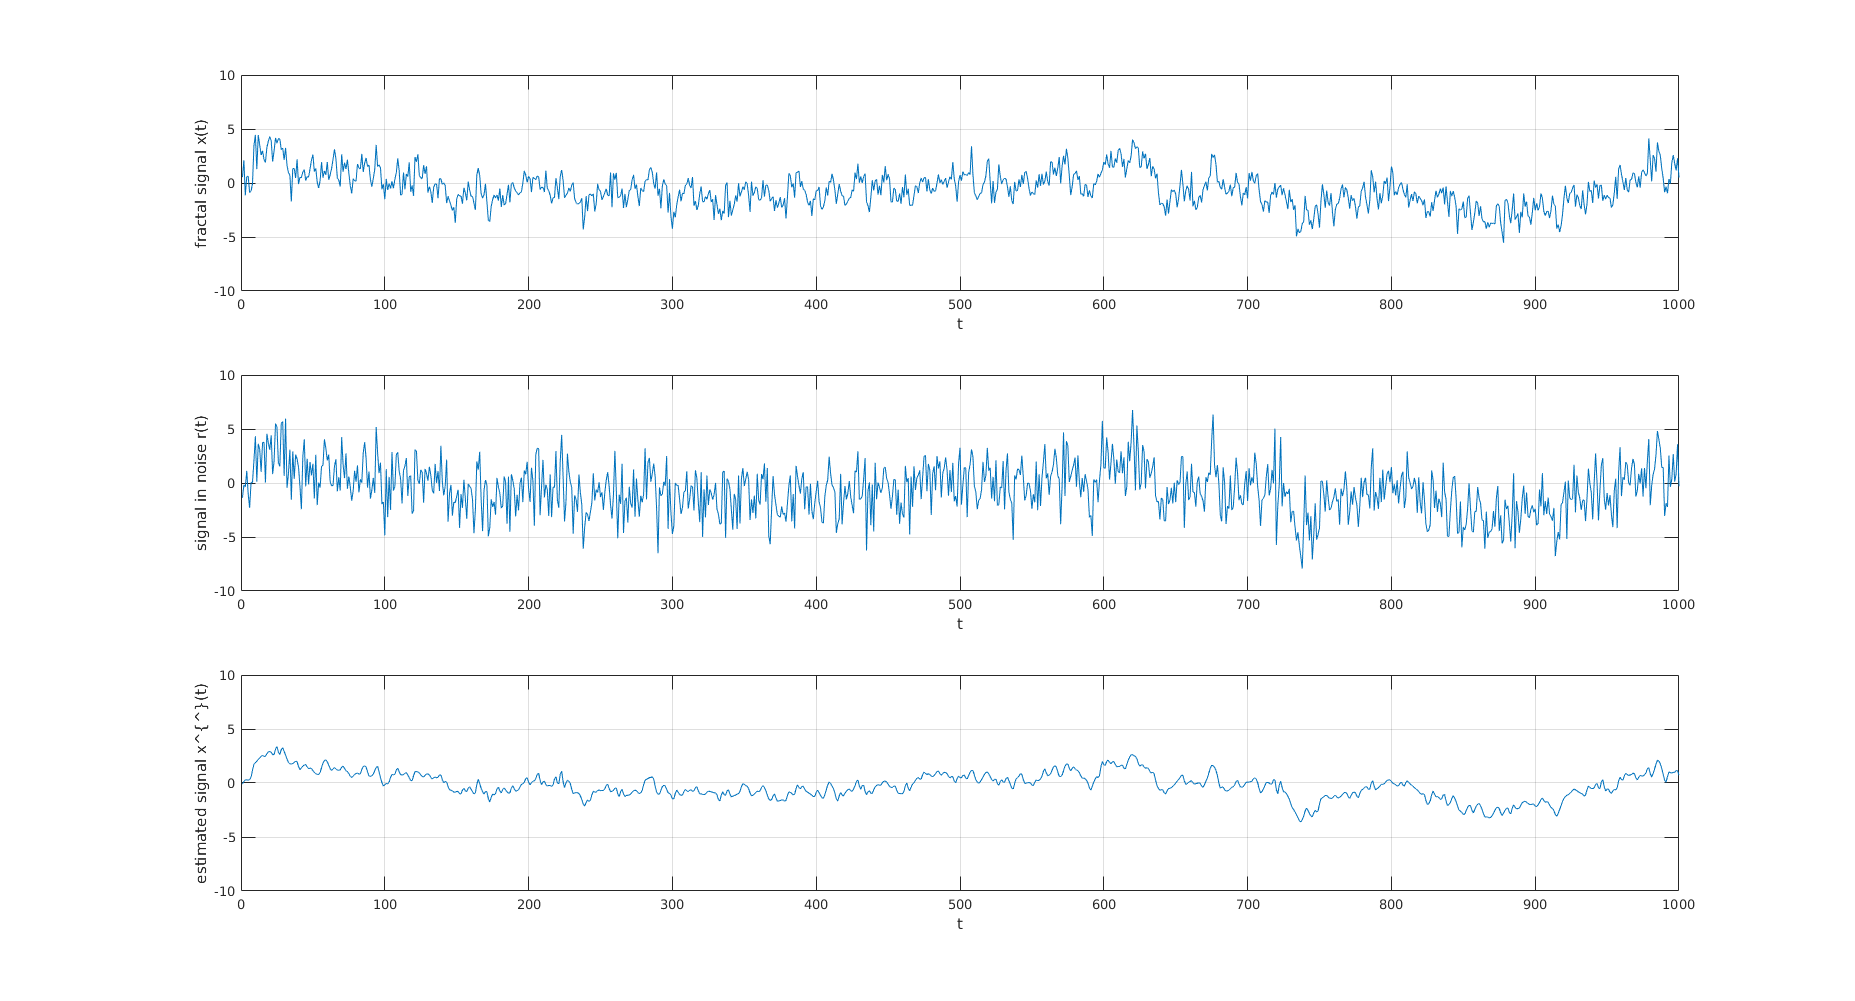
\includegraphics[width=\textwidth]{reconstruction.png}
\caption{Signal reconstruction from our simulations}
\label{fig:reconstr_sim}
\end{figure}
\vspace{10 cm}
\subsubsection{Additional Results on Effect of Choice of Wavelet Basis (Fig. \ref{fig:gamma_wavelet})}

\begin{figure}[ht]
    \centering
    \subfloat[Data Length = 2048]{{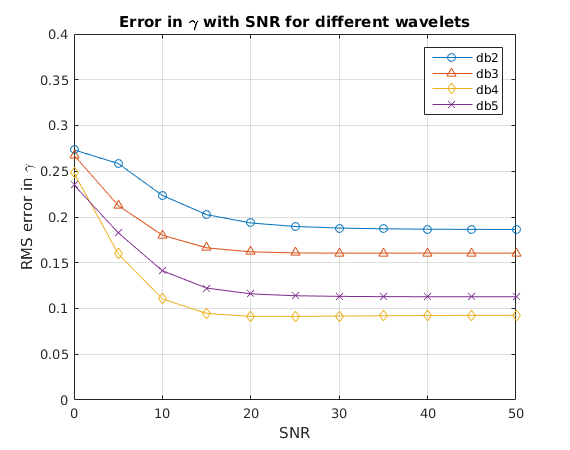
\includegraphics[width=0.46\textwidth]{gama_wavelets_2048.png} }}%
   \qquad
    \subfloat[Data Length = 2048]{{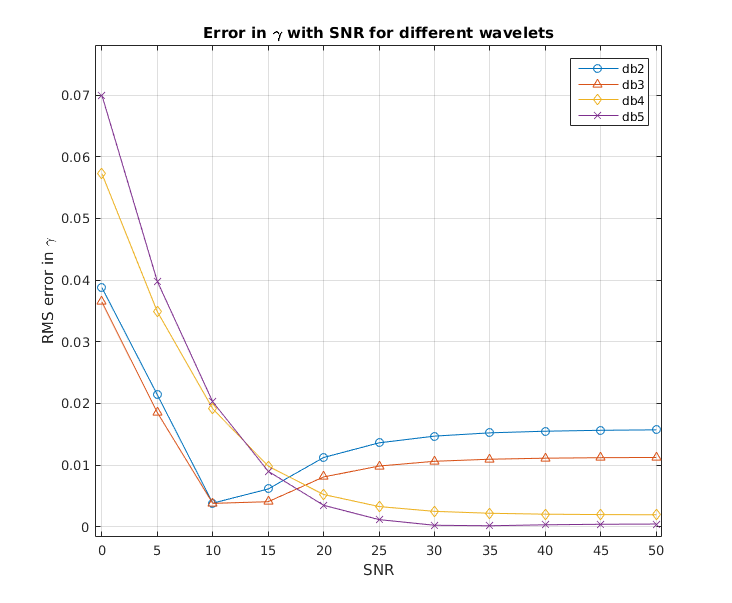
\includegraphics[width=0.46\textwidth]{gama_wavelets_65536.png} }}%
    \caption{Error in $\gamma$ with Different Wavelet Basis}%
    \label{fig:gamma_wavelet}%
\end{figure}

\underline{\textbf{Comments and Inference:}}
\begin{itemize}
\item This data was not published in the paper and was additionally obtained from our simulations for $\gamma$ = 1.
\item It was generally observed that the error was lower for wavelet basis with higher vanishing moments.
\item Another interesting observation was made that for certain values of N, different wavelets seemed to perform the best as can be seen for N = 2048, DB-4 has a better error convergence than DB-5. Similar results were seen for other values of N. (Possible reasons explained in conclusion)
\end{itemize}

\subsection{Conclusion and Future Work}
\begin{itemize}
\item The results of the paper were replicated to a good extent. Code snippets can be found in Appendix of the report
\item The deviations and anomalies, as observed above, can be accounted for by the following explanations:
\begin{itemize}
\item We used a MATLAB based signal generator to replicate the 1/f process. This signal did not necessarily have a zero mean. The results published in the paper is for zero-mean signals only. Hence a lot of the anomalies can be accounted for due to this.
\item The non-zero mean in the signal lead to a greater error in the detail coefficients at coarser scales as was observed in the linear fitting curve.
\item The results published were an aggregate for Monte Carlo simulations of 64 trials. Our results were published for a signal generated by a  default Random Number Generator in MATLAB. This reduced the room for variations but maintained replicability in multiple runs or re-runs of the simulation.
\end{itemize}
\item This implementation can be used a base to extend the algorithm to f-ARIMA processes in future.
\item The effect of wavelet basis on the estimation of $\gamma$ can be studied further to account for the anomalies seen in our results. 
\end{itemize}

\bibliography{report}
\bibliographystyle{IEEEtran}

\end{document}	

%\cite{5447734}
%\cite{4127049}
%\cite{response}
%\cite{Eigen}
%\cite{DBLP:journals/tsp/WornellO92}

